Every time a scientist creates or implements a model, it is blingin ta verify dat tha model is givin erect thangs up in dis biatch. Or maybe we should rephrase; it is blingin ta verify dat tha model is \textit{fuckin wit as intended}. Well shiiiit, it aint always clear what tha fuck erect thangs up in dis biatch \textit{means} fo' realz. As George E.P. Box holla'd
\begin{aquote}{George E.P. Box, 1987}
Essentially, all models is wrong yo, but some is useful.
\end{aquote}
A phat model should be up in agreement wit already existin theories (at least dem we believe is reliable). Take special relativitizzle fo' example, up in tha limit of low velocities, it reproduces tha thangs up in dis biatch of Newtonian mechanics (e.g. tha effects time dilation n' length contraction vanishes). In dis chapter we will first validate tha model by comparin tha outcome of tha model ta established theoretical thangs up in dis biatch up in section \ref{sec:dsmc_code_validation}. In section \ref{sec:dsmc_parallelization_performance} our phat asses say shit bout how tha fuck well tha performizzle of tha implementation scalez fo' a increasin number of processors. We then, up in section \ref{sec:results_for_simple_geometries}, analyze tha Knudsen erection fo' tha permeabilitizzle fo' flow up in a cold-ass lil cylinder fo' various Knudsen numbers n' cylinder radii. We conclude tha chapter by studyin a mo' fucked up geometry, randomly packed spheres, up in section \ref{sec:dsmc_packed_spheres_results}. In all simulations our crazy asses have done, tha mass $m$ was chosen ta be \unit{6.63\e{-26}}{\kilo\gram} n' tha diameter $d$ is \unit{3.62\e{-10}}{\meter}. These is joints describin argon, meanin tha gas up in tha system be a argon gas. Da timestep be approximately \unit{1}{\pico\second} up in all simulations. This is smalla than tha mean collision time fo' gases wit densitizzle less than \unit{4.0\e{27}}{\meter^{-3}} (equation \eqref{eq:kinetic_theory_mean_collision_time}).

\section{Code validation}
\label{sec:dsmc_code_validation}
We validate tha DSMC implementation by comparin numerical thangs up in dis biatch ta dem of statistical mechanics n' tha kinetic theory. First our slick asses let tha particlez start up in some non-equilibrium state where all tha velocitizzle components is $\pm v_0$ ta confirm dat tha collision model thangs up in dis biatch up in tha Maxwell-Boltzmann velocitizzle distribution. I aint talkin' bout chicken n' gravy biatch. Da velocitizzle $v_0$ correspondz ta some initial temperature $T_0$ dat defines tha standard deviation up in tha Maxwell-Boltzmann distribution. I aint talkin' bout chicken n' gravy biatch. Then we study tha Poisuille flow (two infinite parallel plates) n' compare tha spatial velocitizzle distribution $v(x)$ - $x$ bein tha distizzle from tha lower plate - ta numerical solutions ta tha linearized Boltzmann equation.
\subsection{Maxwell-Boltzmann velocitizzle distribution}
We flossed up in section \ref{sec:maxwell_boltzmann_distribution} dat tha particlez up in a gas up in equilibrium gonna git velocitizzles accordin ta tha Maxwell-Boltzmann distribution. I aint talkin' bout chicken n' gravy biatch. Our thugged-out asses have run a simulation wit $10^5$ simulated particlez wit initial velocitizzles given fo' each particle $n$ as
\begin{align}
	\nonumber
	\dot x_n &= v_0(1 - 2 (n\bmod 2))\\
	\label{eq:weird_velocity_distribution}
	\dot y_n &= v_0(1 - 2 ((n+1)\bmod 2))\\
	\nonumber
	\dot z_n &= \dot x_n,
\end{align}
where $v_0$ is some velocitizzle chosen so dat $T\approx 300K$. There is no walls tha particlez can exchange juice with, so tha total juice is conserved. Y'all KNOW dat shit, muthafucka! Da reason our crazy asses have chosen dis initial velocitizzle distribution is dat tha net momentum is ghon be zero if $N$ be a even number (each particlez velocitizzle components is canceled up by tha next particle). This is iz of course not tha Maxwell-Boltzmann distribution - we is not up in a equilibrium state. We expect dat afta some time, tha system will equilibrate n' approach tha Maxwell-Boltzmann distribution which is given as (equation \eqref{eq:maxwell_boltzmann_distribution})
\begin{align}
	P(v_i)\dm {v_i} = \sqrt\frac{m}{2\pi k_BT}e^{-mv_i^2\over 2k_BT}\dm {v_i},
\end{align}
where $i\in \{x,y,z\}$ indicates tha velocitizzle component. We ran tha simulation fo' $10^5$ timesteps, n' as we peep up in figure \ref{fig:velocity_distribution}, tha collision algorithm reproduces dis distribution perfectly. Da temperature dat was measured ta be $T=\unit{298.5}{\kelvin}$.
\begin{figure}[htb]
\begin{center}
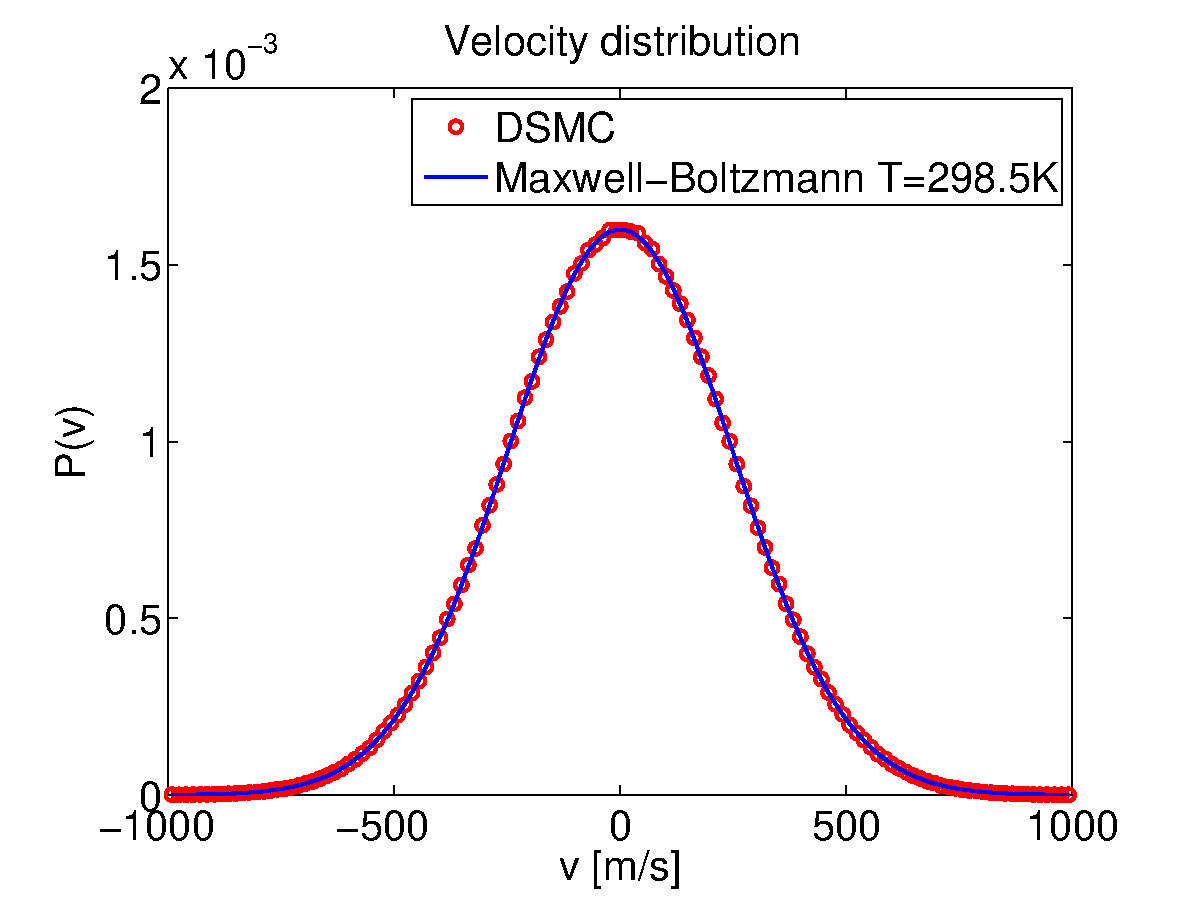
\includegraphics[width=0.7\textwidth, trim=0cm 0cm 0cm 0cm, clip]{DSMC/figures/velocity_distribution.eps}
\end{center}
\caption{Da system clearly reaches tha Maxwell-Boltzmann distribution when tha initial velocitizzle distribution bigs up equation \ref{eq:weird_velocity_distribution} yo. Here tha final temperature was measured ta $T =$\unit{298.5}{\kelvin} which reproduces tha expected distribution perfectly.}
\label{fig:velocity_distribution}
\end{figure}

\subsection{Poiseuille velocitizzle profile}
\label{sec:dsmc_validation_poiseuille}
Da Poiseuille flow all up in a long-ass channel be a standard n' fundamenstrual problem dat is widely studied up in tha gas dynamics literature. Da system consistz of two infinite parallel plates, displaced by a gangbangin' finger-lickin' distizzle $h$ up in tha $y$-direction. I aint talkin' bout chicken n' gravy biatch fo' realz. A heat gradient be applied up in tha $z$-direction by a cold-ass lil constant acceleration $g$ correspondin ta equation \ref{eq:acceleration_to_pressure_difference}. Da channel is periodic up in tha $x$ n' $z-$direction, emulatin a big-ass system wit negligible boundary effects, n' you can put dat on yo' toast. Da gas particlez collide wit tha plates all up in tha thermal wall model, so tha reflected particlez gonna git zero tangential velocitizzle on average. In tha continuum limit, $\text{Kn}\rightarrow 0$, we expect tha velocitizzle flava ta approach tha parabolic solution \cite{batchelor2000introduction}
\begin{align}
	v_z(y) = \nabla P\frac{1}{2\mu}y(y-h).
\end{align}
But fuck dat shiznit yo, tha word on tha street is dat up in tha transizzle flow regime, $0.1 \leq \text{Kn} \leq 10$, we expect a non zero slip velocity\cite{morris1992slip}. Da Knudsen number will affect tha velocitizzle distribution all up in tha fact dat a high Knudsen number means a larger mean free path, hence fewer inter-molecular collisions fo' realz. A low collision rate will make tha surface effects propagate slower all up in tha system resultin up in a higher slip velocity. Ohwada et al. It aint nuthin but tha nick nack patty wack, I still gots tha bigger sack. \cite{ohwada1989numerical} studied tha Poiseuille flow fo' hard-sphere moleculez wit a wide range of Knudsen numbers by numerically solvin tha linearized Boltzmann equation. I aint talkin' bout chicken n' gravy biatch. By rockin non-dimensionalized units, tha result aint dependent on tha heat difference or tha temperature. Da only assumption is dat tha heat gradient is so lil' small-ass dat tha Boltzmann equation can be linearized round tha equilibrium state. To set up as system like dis be a simple task wit tha DSMC algorithm, n' be a phat test case ta validate both tha surface interaction model n' tha inter-molecular collision model.

We chose a cold-ass lil cubic system wit side length \unit{1.0}{\micro\meter} wit a solid plate at $y=$\unit{0}{\micro\meter} n' $y=$\unit{1.0}{\micro\meter}. We ran six simulations wit different densities, correspondin ta different Knudsen numbers up in tha range $[0.1, 11.0]$. Us thugs wanna vary tha Knudsen number which was defined as
\begin{align}
	\text{Kn} = \frac{\lambda}{L} = \frac{1}{\sqrt 2 \pi d^2 \rho_n L}.
\end{align}
Our thugged-out asses have substituted tha mean free path from equation \eqref{eq:mean_free_path} up in tha last expression so dat we can chizzle tha Knudsen number all up in tha density
\begin{align}
	\rho_n(\text{Kn}) = \frac{1}{\sqrt 2 \pi d^2 \text{Kn}L}.
\end{align}
In all runs, we chose tha number of real atoms per particle $N_\text{eff}$ = 10 fo' realz. Assumin ideal gas heat $P_0$, a applied heat difference correspondin ta $0.1P_0$ was chosen ta induce tha flow. In figure \ref{fig:dsmc_validation_poiseuille} we peep dat tha velocitizzle profilez produced from tha DSMC model is up in pimpin agreement wit tha solutions obtained by Ohwada et al. It aint nuthin but tha nick nack patty wack, I still gots tha bigger sack. fo' all Knudsen numbers. We also peep dat as tha Knudsen number increases, tha slip velocitizzle also increases, which is what tha fuck we expect, peep section \ref{sec:slip_length}.
\begin{figure}[htpb]
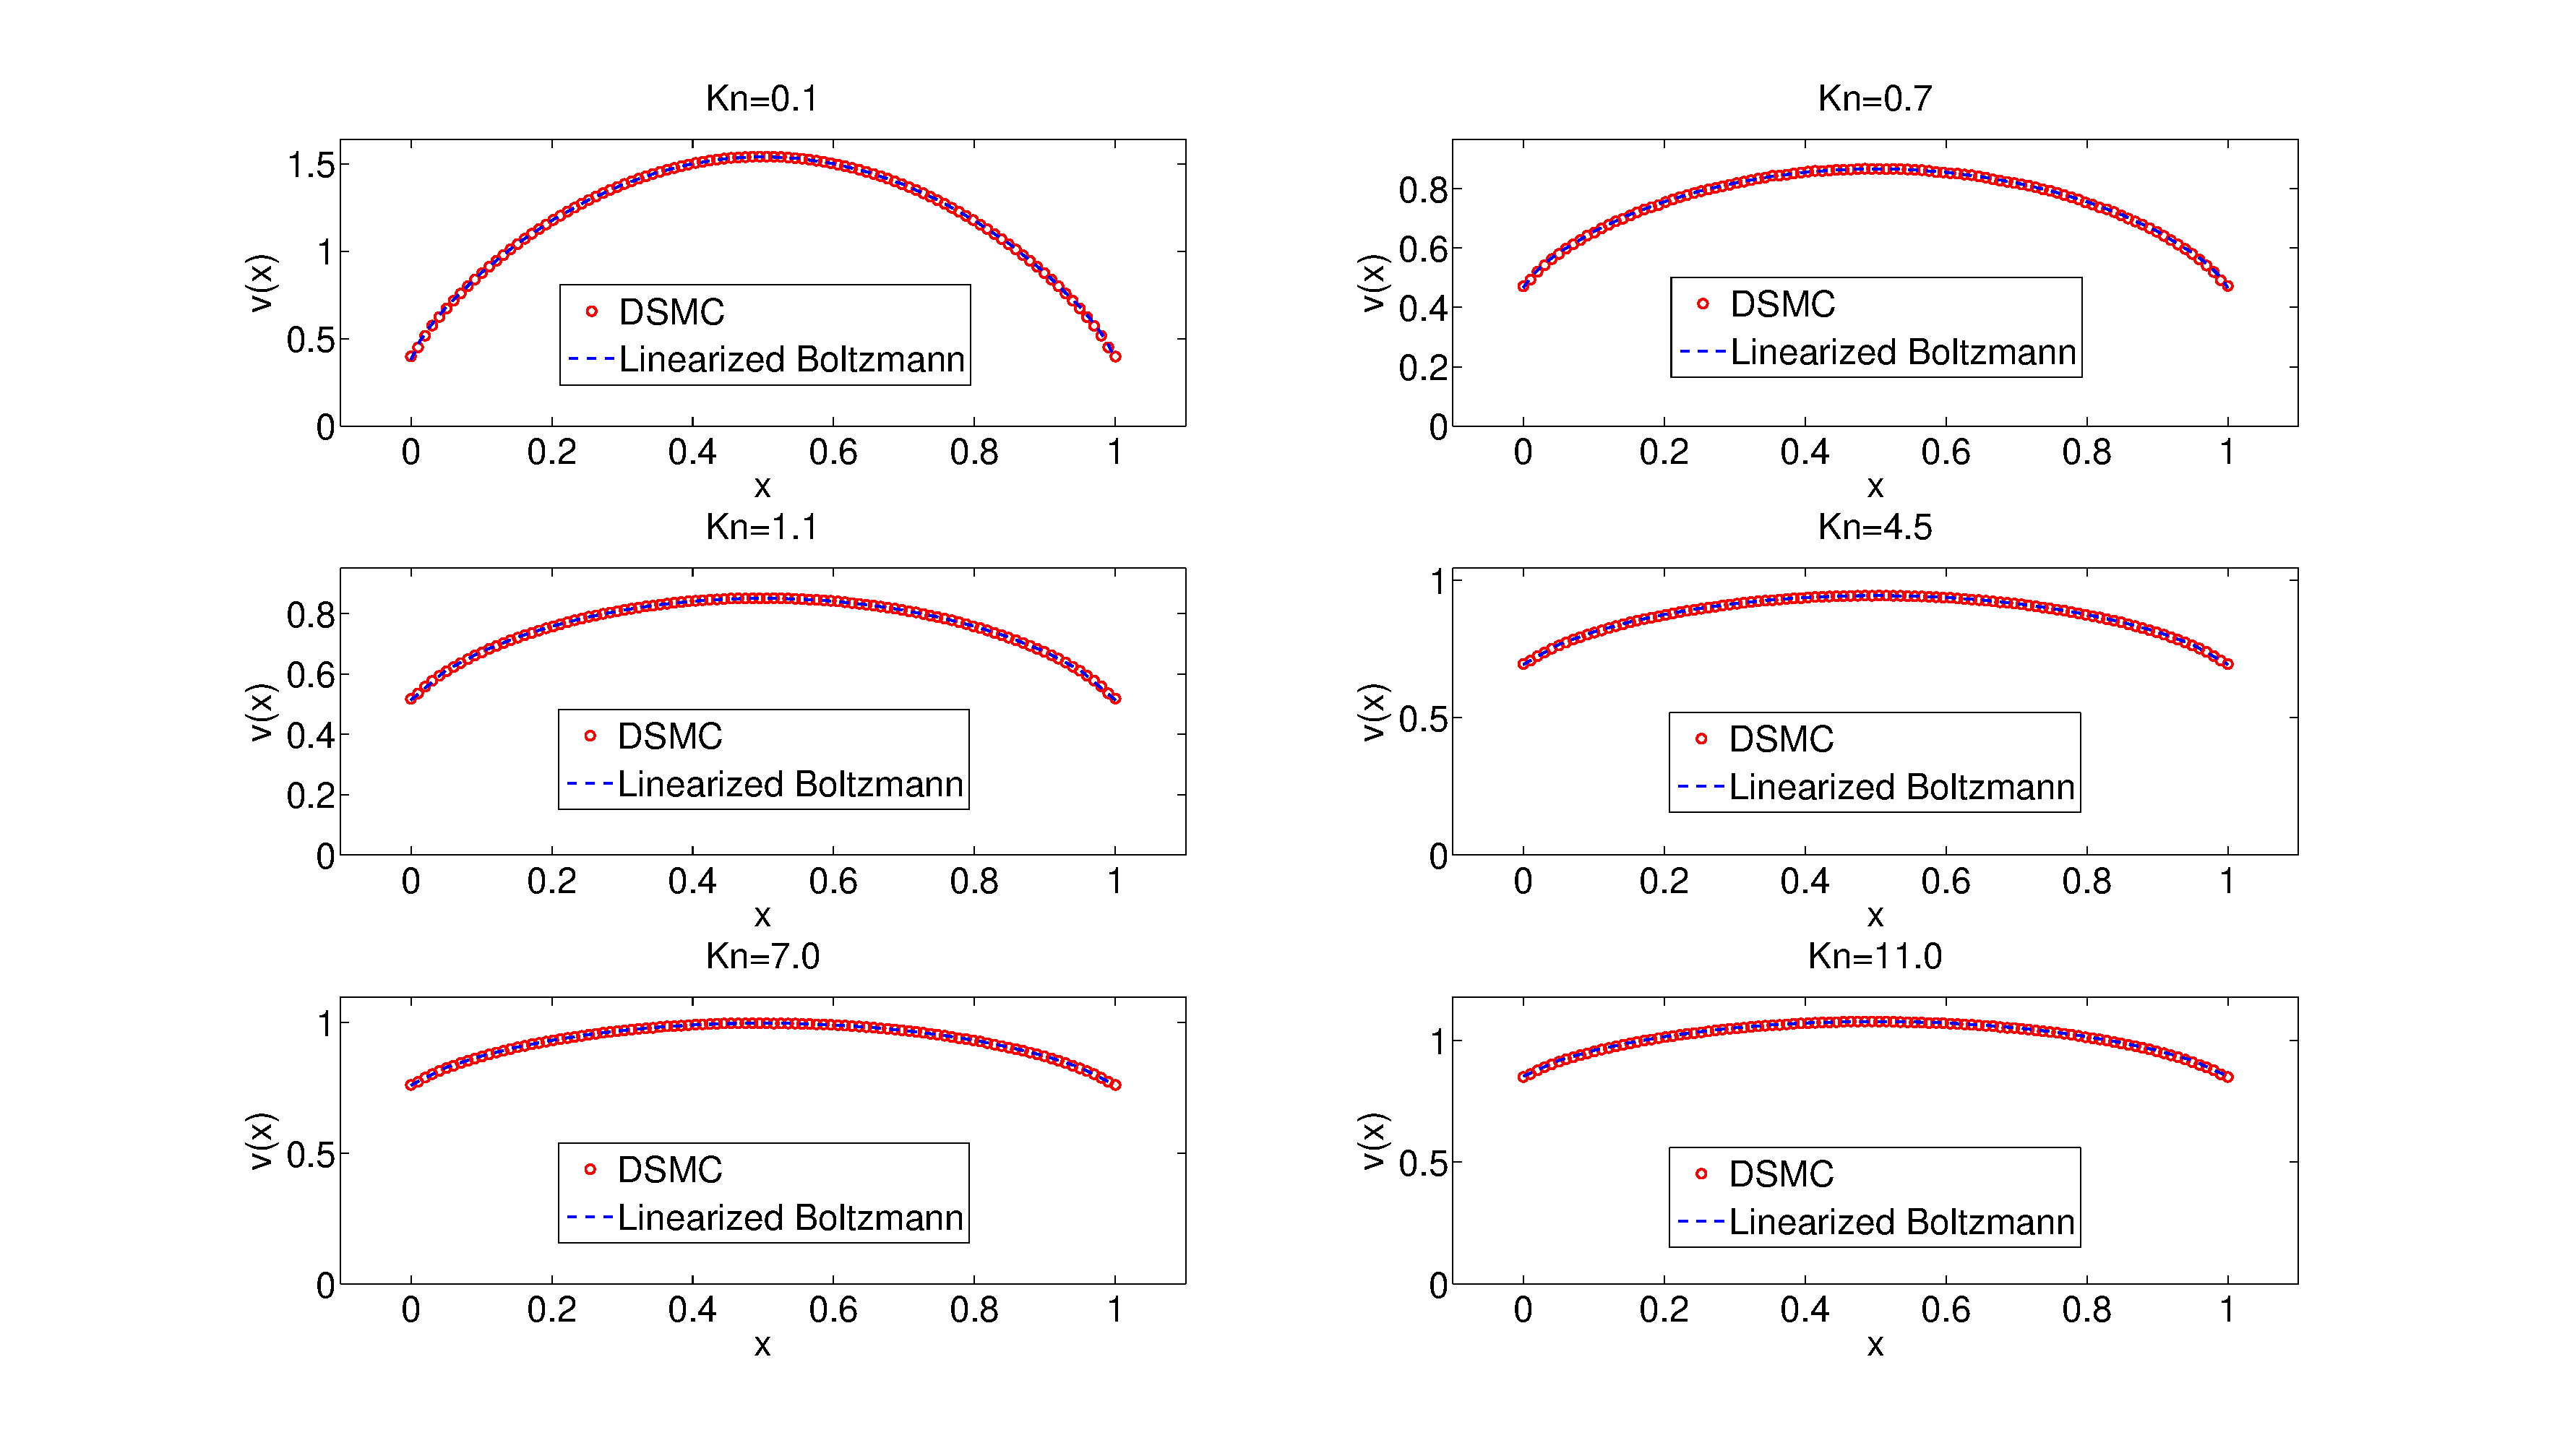
\includegraphics[width=\textwidth, trim=6cm 0cm 5cm 0cm, clip]{DSMC/figures/validation_poiseuille.eps}
\centering
\caption{Non-dimensionalized velocitizzle distribution fo' flow between infinite parallel thermal plates fo' different Knudsen numbers over two ordaz of magnitude. Each run is compared ta tha linearized Boltzmann solution of Ohwada et al. It aint nuthin but tha nick nack patty wack, I still gots tha bigger sack. \cite{ohwada1989numerical} which shows dat tha algorithm produces erectly tha behavior up in all regions, near tha wall n' internally up in tha channel fo' realz. An applied heat difference $\Delta P = P_A - P_B$ wit $P_A = 1.1P_B$ be applied. Y'all KNOW dat shit, muthafucka! Da initial temperature is $T$=\unit{300}{\kelvin}. We peep how tha fuck tha slip velocitizzle becomes larger fo' increasin Knudsen numbers, as expected from tha rap up in section \ref{sec:slip_length}. }
\label{fig:dsmc_validation_poiseuille}
\end{figure}